\RequirePackage{cdo}
\title{Notes Projet}
\author{Groupe 3}

\begin{document}
\maketitle

\section*{Principe du jeu}

Ce jeu de coopération entre 2 joueurs se déroule dans un donjon. Le donjon est constitué de 3 étages (chacun généré aléatoirement) pour chaque étage, une salle contient la clé pour accéder à la salle du Boss. Pour gagner il faut vaincre les Boss de chacun des étages.

\section{Joueurs}

Les joueurs doivent coopérer pour gagner. Si un joueur meurt la partie est perdue. Si les joueurs parviennent à tuer le 3éme Boss alors la partie est gagnée. Un joueur se bat au corps à corps (CàC) et l'autre joueur à distance.

\subsection*{Lampe à huile (torche)}

Une seule lampe à huile partagée par les 2 joueurs. Le fait de porter la torche augmente le champ de vision de l'utilisateur mais l'empêche d'utiliser les armes à deux mains et le ralenti. La torche peut être échangée entre les 2 joueurs.

\subsection*{Possession}

Les joueurs peuvent prendre possession de l'ennemi le plus proche (sauf Boss). Pendant cette possession le corps du joueur disparaît, si l'ennemi meurt alors le joueur meurt (Game over). Si le joueur avec la torche réalise la possession alors la torche s'éteint.

\section{Ennemi (mobs)}

\subsection*{Ennemi classique}

Le jeu possède plusieurs ennemis, dont un ennemi type slime qui se divise en 2 slimes plus petit à sa mort jusqu'à disparaître.

\subsection*{Boss}

Les Boss possèdent des salles réservées, les joueurs sont bloqués dans la salle du Boss jusqu'à son élimination. Une fois le Boss éliminé, les joueurs peuvent retourner en arrière (Ouverture de la porte) et la porte de changement d'étage apparaît.

Les salles de Boss possèdent un biome (terrain) différent, par exemple la présence d'eau, sable affectant les déplacements des joueurs.

\section{Étage}

Le donjon est constitué de 3 étages. Chaque étage est généré aléatoirement avec des salles de mobs (ennemis), des salles d'énigmes, une salle contenant la clé pour accéder au Boss et la salle du Boss. Lorsque un joueur entre dans une porte, les 2 joueurs sont téléportés dans la nouvelle salle dans laquelle ils doivent éliminer toutes les entités hostiles pour ouvrir les portes voir la \rfss{TP}. Cependant il est impossible de retourner à l'étage précédent une fois la porte de fin d'étage passée.

\subsection*{Salle énigme}

Pour les salles avec les énigmes, des spawners sont présents, qui font apparaître des entités neutres utiles à la résolution de l'énigme (Utilisation de la possession). 

\subsection*{Génération des salles}

Pour la génération des étages nous avons 2 idées d'implémentations principales :

\begin{itemize}
\item Solution préférable (pour la qualité du jeu) :
Les salles sont préfaites et on les places aléatoirement avec des liaisons par couloirs. Toutes les salles placées sont alors accessibles mais ne sont pas forcement utiles.

\item Autre solution :
Une grille dont chaque case représente l'unité de mesure minimale d'une salle. Une salle est alors un ensemble de cases de la grille.
\end{itemize}

\section{Camera}

Centré sur le centre des 2 joueurs la caméra possède une taille fixe voir \rfss{Viewport}. Si la caméra "déborde" sur une autre salle alors la salle voisine est affichée en assombri (sans la torche).

\section{ATH}

En haut de l'écran on affiche en superposé sur le terrain de jeu :

\begin{center}
\begin{tabular}{l|p{2cm}|c|p{2cm}|r}
HP J1 & & Combustion Torche & & HP J2 \\
\end{tabular}
\end{center}

\section{Optionnel}

\subsection*{TP des joueurs}
\label{subsec:TP}

Les joueurs sont désormais téléportés (TP) automatiquement dans les nouvelles salles avec des mobs (qui doit donc être fermée).

\subsection*{Viewport}
\label{subsec:Viewport}

La caméra s'agrandit quand les joueurs s'éloignent l'un de l'autre, et inversement elle se réduit lorsque les joueurs se rapprochent. La caméra possède un seuil de zoom minimal et maximal, si les joueurs essaie de sortir du zoom minimal alors leurs mouvements sont entravés.

\subsection*{Épuisement de la torche}

L'efficacité de la torche diminue avec le temps jusqu'à s'éteindre. Il est alors possible de la recharger dans une salle spéciale  l'étage.

\subsection*{Système de classe}

En début de partie les joueurs sont des aventuriers. Une fois le premier Boss vaincu les joueurs peuvent choisir une classe. Après le deuxième Boss, les joueurs peuvent choisir une spécialisation de leur classe.

\begin{center}
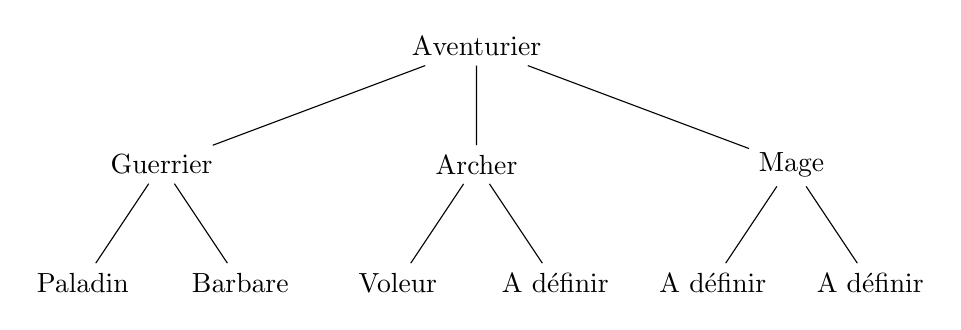
\begin{tikzpicture}[level 1/.style={sibling distance=4cm}, level 2/.style={sibling distance=2cm}]
\node {Aventurier}
child {node {Guerrier}
	child {node {Paladin}} child {node {Barbare}}}
child {node {Archer}
	child {node {Voleur}} child {node {A définir}}}
child {node {Mage}
	child {node {A définir}} child {node {A définir}}};
\end{tikzpicture}
\end{center}

\subsection*{Loots d'armes}

Des armes sont disponibles dans le donjon avec des statistiques différentes (vitesse, dégât).

\subsection*{Compétences}

Liés aux classes à définir.

\subsection*{Mini Map}

Implémentation d'une minimap à ajouter à l'ATH

\end{document}
